\section{Future Work}

\newpar Extending the implementation of the EBA analyzer has proven to be a relatively fast approach for developing error checkers analyzing the Linux kernel, allowing building an error checker that is able to process these files with relative ease. 

\newpar Implementing error checkers for other error types would allow the EBA analyzer to possibly detect more error types when validate the source code for Linux components. Extending the analyzer in this way allows the user(s) of the analyzer to check for specific error types, speeding up evaluation of source code if specific error checks are desired. 

\newpar Implementing the prototype checker using a monitor state machine instead of the limited subset of CTL could potentially result in an implementation with greater accuracy. The implementation of such an approach might prove easier to reason about and debug, though it is unknown if this is the case. An example of such a state machine can be seen in Fig. \ref{fig:statemachine}. The CTL format properties of the existing checkers can also be implemented as monitor state machines and therefore implemented as automata algorithms. I believe the CTL-inspired implementation of this project can be translated into a finite state machine, though this would have to be determined in a future project. 

\begin{figure}[h]
    \centering
    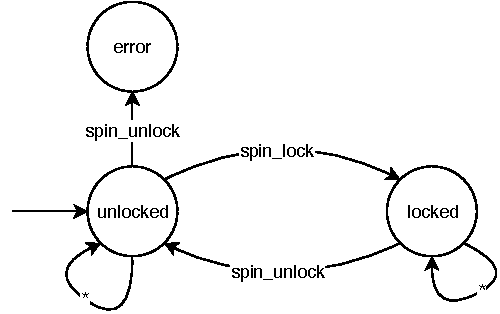
\includegraphics[width=0.35\textwidth]{futurework/figures/state-machine}
    \caption{An example of a double-unlock monitor state machine.}
    \label{fig:statemachine}
\end{figure}

\newpar Implementing the shortcomings of the prototype of this project explained in the previous section in order to detect a larger number of true positives should be done by improving the ability of the implementation of the EBA analyzer to detect unlock statements in the source code. This would improve the accuracy and therefore the usefulness of the prototype.

\newpar Another improvement to the analyzer would be to improve the parsing of the input files. The \texttt{eba-cil} library used for generating the C intermediate language used by EBA does currently not support constructs found in the output of the GCC compiler heavily used by the Linux kernel developers. These include:
\begin{itemize}
    \item \textit{Static Assertions}, added in C11 which has been implemented since since GCC 4.6\footnote{See \textit{Programming Languages - C} \cite{ISO:2011:IIIb}}
    \item \textit{Assembler Instructions with C Expression Operands}, an extension available since GCC 3.1\footnote{See \textit{Assembler Instructions with C Expression Operands} \cite{GCC:3.1}}
\end{itemize}

\noindent Currently the output from GCC on input files using these features results in a parse error in EBA and therefore need to be removed from the compiler output before analysis. This negatively impacts the soundness of the analysis due to the removal of source code. Supporting these features in the implementation of EBA would improve the soundness of the analysis.